\documentclass[10 pt,usenames,dvipsnames, oneside]{article}
\usepackage{../../../modelo-ensino-medio}



\begin{document}

\begin{center}
  \begin{minipage}[l]{3cm}

\includegraphics[width=2cm]{logo}    
\end{minipage}\hfill
\begin{minipage}[r]{.8\textwidth}
 {\Large \scshape Atividade: Carrinho VertiGo}  
\end{minipage}
\end{center}
\vspace{.2cm}

\ifdefined\prof
%Habilidades da BNCC
% \begin{objetivos}
% \item 
% \end{objetivos}

%Caixa do Para o Professor
\begin{goals}
%Objetivos específicos
\begin{enumerate}
\item Introduzir a ideia e a construção da Função de Euler,
\item Estabelecer a relação entre números reais e pontos de uma circunferência unitária.
\end{enumerate}

\tcblower

%Orientações e sugestões
\begin{itemize}
\item Sugerimos ao professor orientar os alunos, se necessário, a observarem que uma distância vertical de comprimento “$a$”{} percorrida pelo carrinho se reflete na posição do selo, o qual se moverá ao longo da roda percorrendo um arco de circunferência de mesmo comprimento “$a$”.
\item  O uso de objetos redondos e barbante utilizados na atividade “Cobrindo circunferências com seus raios”{} pode ajuda-los nessa percepção.
\end{itemize}
\end{goals}

\bigskip
\begin{center}
{\large \scshape Atividade}
\end{center}
\fi

\begin{quote}

Pesquisadores da Disney Research, em parceria com o Instituto Federal de Tecnologia de Zurique, demonstraram esta semana um carrinho de quatro rodas capaz de escalar paredes e andar normalmente em superfícies verticais.
À primeira vista, parece um brinquedo, mas, segundo os criadores, a tecnologia pode ampliar os limites de exploração para equipamentos robóticos. Batizado como VertiGo, o carrinho é “capaz de mover em uma parede rapidamente e com agilidade”, informam os pesquisadores. Para realizar a façanha, ele possui duas hélices propulsoras móveis que fornecem o impulso necessário para o início da escalada e, depois, mantém o VertiGo junto à parede.”

\flushright
Fonte: \href{https://gizmodo.uol.com.br/o-novo-robo-da-disney-escala-paredes-como-uma-lagartixa/}{Gizmodo}
\end{quote}


\begin{figure}[H]
\centering

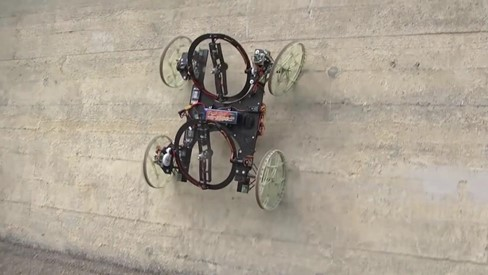
\includegraphics[width=.7\linewidth]{trigonometricas45}
\end{figure}

Neste link é possível ver o VertiGo em ação: \url{https://www.youtube.com/watch?v=KRYT2kYbgo4}


Suponha que foi colado um pequeno selo em uma das rodas do VertiGo. O carrinho começará a descer em um paredão vertical bem alto, seguindo um caminho reto e paralelo ao paredão. Ele começa o movimento “colado”{} ao paredão, quando o selo está em contato com o mesmo. Conforme o carrinho vai descendo, o selo se movimenta conforme o giro da roda. A figura abaixo ilustra o movimento realizado por essa roda ao descer o paredão e os pontos $A_1$, $A_2$ e $A_3$ ilustram posições do selo ao longo do movimento. Suponha que o raio da roda seja de $1$ dm

\begin{figure}[H]
\centering

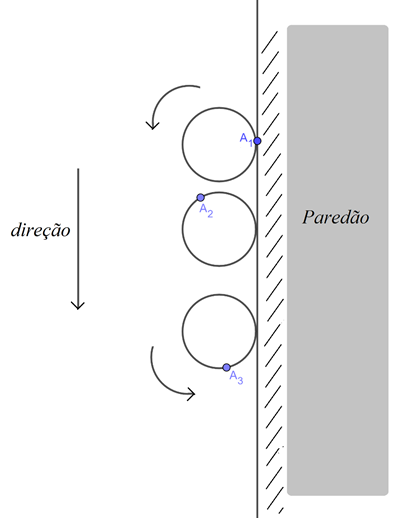
\includegraphics[width=.375\linewidth]{trigonometricas46}
\caption{Fonte: Adaptado de Ekici (2010)}
\label{trigonometrica46}
\end{figure}

\begin{enumerate}
\item Indique a posição do selo na circunferência da roda quando o VertiGo tiver descido as seguinte distâncias:

$0\text{ dm}, 1\text{ dm}, 2\text{ dm}, \frac{3}{2}\text{ dm}, \frac{\pi}{2}\text{ dm}, \pi\text{ dm}, 3\pi\text{ dm}, 2\pi\text{ dm}, 7\text{ dm}, 4\text{ dm}$
\item Suponha que, do ponto de repouso do VertiGo, agora ele irá \textbf{subir} parte do paredão. Usando a mesma vista lateral dada pela \fref{trigonometrica46}, qual será a posição do sela para as mesmas medidas do item \titem{a)}?
\end{enumerate}

\ifdefined\prof
\begin{solucao}

\begin{enumerate}
 \item A posição do selo referente às distâncias $0, 1, 2, \frac{3}{2}, \frac{\pi}{2}, \pi, \frac{3\pi}{2}$ e $7$ dm estão representadas  no desenho abaixo respectivamente pelos pontos $A_1, A_2, A_3, A_4, A_5, A_6, A_7\text{ e }A_8$. A posição referente às distâncias $2\pi$ e $4\pi$ dm é mesma do ponto $A_1$

 \begin{figure}[H]
 \centering
 
 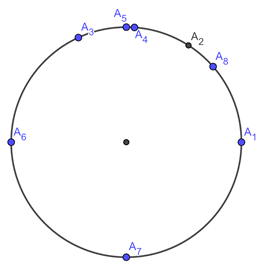
\includegraphics[width=.4\linewidth]{trigonometricas47}
 \end{figure}
 \item Basta refletir os pontos obtidos no item \titem{a)} relativamente à reta horizontal que passa pelo centro da circunferência e o ponto $A_1$.
 \end{enumerate}

\end{solucao}
\fi

\end{document}